\documentclass[UTF8]{ctexart}
\usepackage{amsmath}
\usepackage{graphicx}
\usepackage{minted}
\usepackage{hyperref}

\hypersetup{hidelinks}

\graphicspath{ {images/} }

\title{数据结构第一次作业}
\date{2016-9-30}
\author{沈俞霖}

\begin{document}
  \maketitle
  \vspace{100mm}
  \begin{flushright}
  \textbf{课程} 数据结构与算法

  \textbf{姓名} 沈俞霖

  \textbf{专业班级} 软件51

  \textbf{学号} 2151601013

  \textbf{邮箱} sylxjtu@outlook.com

  \textbf{提交日期} 2016-10-*
  \end{flushright}
  \newpage

  \tableofcontents
  \newpage

  \section{复杂度与时间估计}
    \subsection{作业题目}
      程序A和程序B经过分析发现其最坏情形运行时间分别不大于 $150N\log N$ 和 $N^2$ 。如果可能,请回答下列问题:
      \paragraph{A}
      对于 $N$ 的大值( $N>10000$ ),哪一个程序的运行时间有更好的保障?
      \paragraph{B}
      对于 $N$ 的小值( $N<100$ ),哪一个程序的运行时间有更好的保障?
      \paragraph{C}
      对于 $N=1000$ ,哪一个程序平均运行得更快?
      \paragraph{D}
      对于所有可能的输入,程序B是否总比程序A运行得快?
    \subsection{问题分析}
      \paragraph{A}
      A程序运行时间有更好的保障。当 $N=10000$ 时,在最坏情况下, $ 150 N \log N \approx 2 \times 10 ^ 7 $ , 而 $ N^2 = 10 ^ 8 $, 故A程序运行时间有更好的保障。
      \paragraph{B}
      B程序运行时间有更好的保障。当 $N=100$ 时,在最坏情况下, $ 150 N \log N \approx 10 ^ 5 $ , 而 $ N^2 = 10 ^ 4 $, 故B程序运行时间有更好的保障。
      \paragraph{C}
      不能判断,因为题目只给出了最坏情况运行时间,没有给出平均情况运行时间。
      \paragraph{D}
      不能判断,因为题目只给出了最坏情况运行时间,不能以此来判断所有的输入。
  \section{递归方程求复杂度}
    \subsection{作业题目}
      考虑以下递归方程,定义函数 $T(n)$ :
      \paragraph{A}
      \begin{equation}
        T(n) =
        \begin{cases}
          1, & \text{如果$n=1$} \\
          T(n - 1) + n, & \text{其他情况}
        \end{cases}
      \end{equation}
      \paragraph{B}
      \begin{equation}
        T(n) =
        \begin{cases}
          1, & \text{如果$n=0$} \\
          2T(n - 1), & \text{其他情况}
        \end{cases}
      \end{equation}

      请给出A和B两种递归式的大O表示,并证明。
    \subsection{问题分析}
      \paragraph{A}
        $T(n) = O(n^2)$

        \subparagraph{证明}

        (1) 令 $n = 1$,
        $$T(n) = 1 = \frac {n^2 + n}{2}$$

        (2) 若
        $$T(k) = \frac {k^2 + k}{2}$$
        则 $T(k + 1) = T(k) + k + 1$, 即
        $$T(k + 1) = \frac {(k + 1)^2 + (k + 1)}{2}$$

        由(1)(2)可知,
        $$T(n) = \frac {n^2 + n}{2}$$
        故 $T(n) = O(n^2)$,证毕。

      \paragraph{B}
        $T(n) = O(2^n)$

        \subparagraph{证明}

        (1) 令 $n = 0$,
        $$T(n) = 1 = 2 ^ n$$

        (2) 若
        $$T(k) = 2 ^ k$$
        则 $T(k + 1) = 2T(k)$, 即
        $$T(k + 1) = 2 ^ {k + 1}$$

        由(1)(2)可知,
        $$T(n) = 2 ^ n$$
        故 $T(n) = O(2 ^ n)$,证毕。
  \section{测试排序算法}
    \subsection{作业题目}

    实现直接插入排序、简单选择排序、希尔排序、快速排序和归并排序,以能够对给定数组的正序排序,并按照满足下列情形进行测试:

      \paragraph{A} 测试数组的大小为[100,200,300,…,10000] 100 种大小

      \paragraph{B} 测试数组中的元素分别为正序、逆序和随机序列

      \paragraph{} 对测试的结果需要用图形的方式进行展示:

        \subparagraph{a} 展示每个排序算法在满足条件 A 和条件 B 情形下的运行时间趋势变化图,如图 1 所示

        \begin{figure}[H]
          \caption{对选择排序的分析}
          \centering
          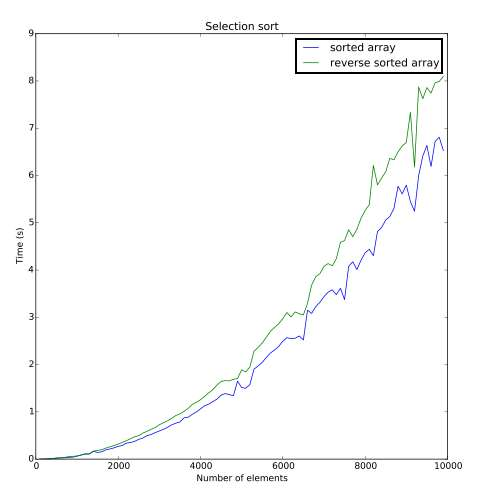
\includegraphics[width=0.5\textwidth]{example1}
        \end{figure}

        \subparagraph{b} 将所有排序算法在正序下、逆序下和随机序列下的运行时间的对比图,如图 2 所示

        \begin{figure}[H]
          \caption{对逆序排序的分析}
          \centering
          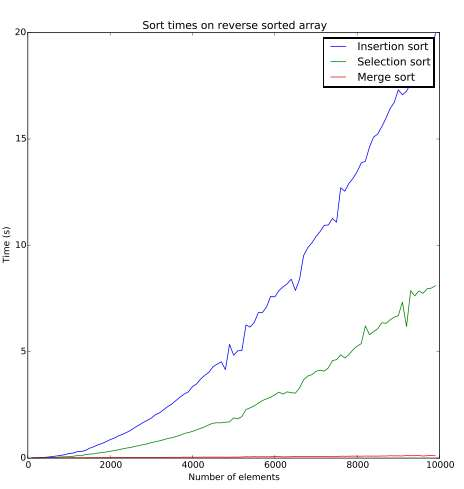
\includegraphics[width=0.5\textwidth]{example2}
        \end{figure}

    \subsection{程序实现}
    仅列出算法代码,完整代码详见
      \href{https://github.com/sylxjtu/datastructure-homework/tree/master/homework1/src}{Github代码仓库}
      \footnote{https://github.com/sylxjtu/datastructure-homework/tree/master/homework1/src}
      \paragraph{插入排序}
      \inputminted{java}{src/InsertionSort.java}
      \paragraph{选择排序}
      \inputminted{java}{src/SelectionSort.java}
      \paragraph{希尔排序}
      \inputminted{java}{src/ShellSort.java}
      \paragraph{快速排序}
      \inputminted{java}{src/QuickSort.java}
      \paragraph{归并排序}
      \inputminted{java}{src/MergeSort.java}

    \subsection{程序运行结果与时间统计}
    \paragraph{运行结果} 所有排序程序全部通过正确性测试
    \paragraph{时间统计} 以图表形式给出,详细数据详见
      \href{https://github.com/sylxjtu/datastructure-homework/blob/master/homework1/data/out.txt}{Github代码仓库}
      \footnote{https://github.com/sylxjtu/datastructure-homework/blob/master/homework1/data/out.txt}
      \subparagraph{a} 每个排序算法在满足条件 A 和条件 B 情形下的运行时间趋势变化图
        \begin{figure}[H]
          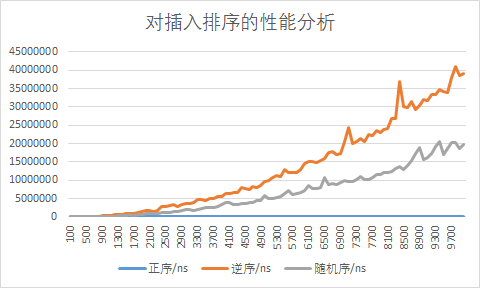
\includegraphics[width=\textwidth]{insertionsort}
          \centering
        \end{figure}
        \begin{figure}[H]
          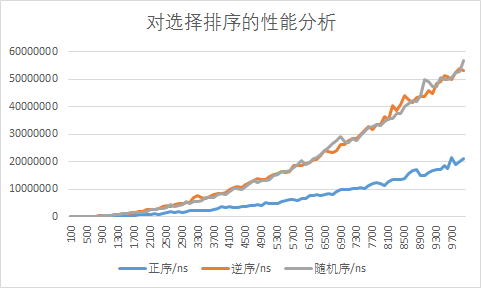
\includegraphics[width=\textwidth]{selectionsort}
          \centering
        \end{figure}
        \begin{figure}[H]
          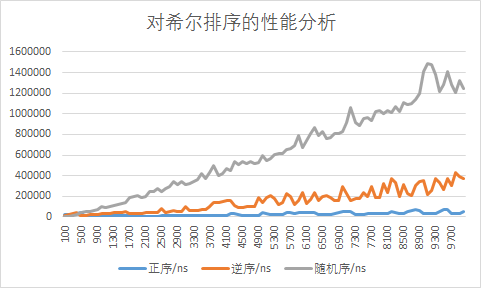
\includegraphics[width=\textwidth]{shellsort}
          \centering
        \end{figure}
        \begin{figure}[H]
          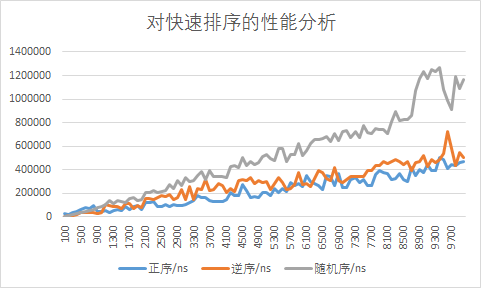
\includegraphics[width=\textwidth]{quicksort}
          \centering
        \end{figure}
        \begin{figure}[H]
          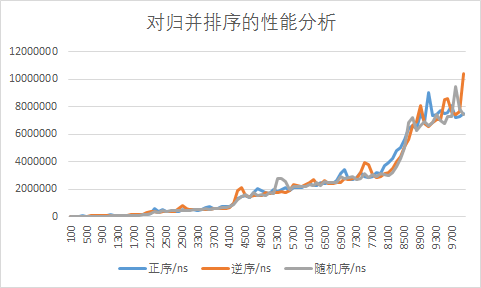
\includegraphics[width=\textwidth]{mergesort}
          \centering
        \end{figure}
      \subparagraph{b} 所有排序算法在正序下、逆序下和随机序列下的运行时间的对比图
        \begin{figure}[H]
          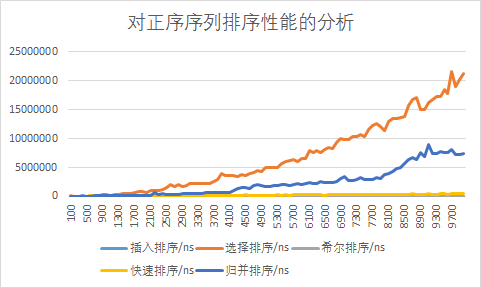
\includegraphics[width=\textwidth]{seq}
          \centering
        \end{figure}
        \begin{figure}[H]
          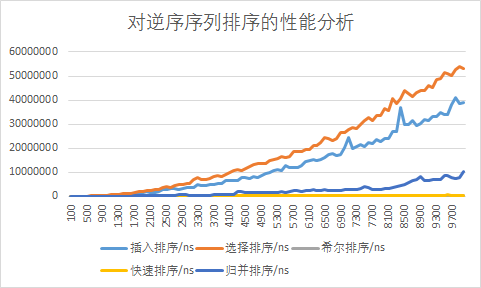
\includegraphics[width=\textwidth]{rev}
          \centering
        \end{figure}
        \begin{figure}[H]
          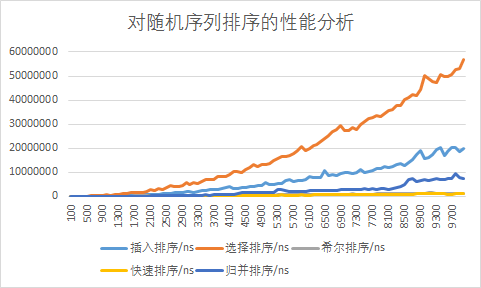
\includegraphics[width=\textwidth]{random}
          \centering
        \end{figure}
    \subsection{算法分析}
      每个算法在不同数据条件下都有一些不同的性能表现,插入排序和希尔排序的性能表现在正序时明显优于其他情况,而归并排序的时间复杂度最为稳定,三种情况下所需时间基本相等。

      在处理大量数据时,希尔排序、快速排序和归并排序速度明显优于插入排序和选择排序的速度,表现了复杂度低的算法在面对大量数据时的优越性。
  \section{选取主元素}
    \subsection{作业题目}
      大小为 $N$ 的数组 A,其主元素是一个出现超过 $N/2$ 次的元素(从而这样的元素最多有一个)。

      例如,数组 3,3,4,2,4,4,2,4,4 有一个主元素 4

      数组 3,3,4,,4,4,2,4 没有主元素。

      使用两种方法实现该问题的求解,并编写程序进行实现。

      同时给出两种求解的算法分析。

    \subsection{程序实现}
      使用了两种求解方法,分别是排序后顺序查找的方法和用哈希表统计后再查找的方法。
      \paragraph{代码}
      \inputminted{java}{src/Problem4.java}

    \subsection{程序运行结果与时间统计}
      \paragraph{运行结果} 两种解法均通过测试
      \paragraph{运行时间} 使用$10 ^ 6$个随机数据进行最坏情况运行时间测试
        \subparagraph{解法1运行时间} $1.86 \times 10 ^ 8$ns
        \subparagraph{解法2运行时间} $8.50 \times 10 ^ 8$ns

    \subsection{算法分析}
      \paragraph{解法1}
        解法1理论复杂度为$O(n\log n)$(排序) + $O(n)$(遍历),即为 $O(n\log n)$。
      \paragraph{解法2}
        解法2理论复杂度为$3nO(1)$(2n次哈希表查找,n次哈希表修改),即为$O(n)$,由于哈希表本身的常数复杂度使得该解法求解较慢。
  \section{选择问题}
    \subsection{作业题目}
      选择问题:在一组数据中选择第 k 大数据的问题。请给出你的解决方法,并给出该解决方案的时间性能分析。
    \subsection{程序实现}
      按照分治的策略,随机选取轴值,把元素划分成小于轴值、大于等于轴值和轴值本身三部分,分类讨论目标元素可能处在的部分,并继续查找。
      \paragraph{代码}
      \inputminted{java}{src/Problem5.java}
    \subsection{程序运行结果与时间统计}
      \paragraph{运行结果} 解法通过了测试,有正确性
      \paragraph{运行时间} $ 10 ^ 6 $ 个数据, $ 100 $ 次查询,最终用时 $3.51 \times 10 ^ 8$ ns
    \subsection{算法分析}
      在平均情况下,对大小为 $n$ 的数组,程序每次运行,都以 $O(n)$ 了复杂度遍历了整个数组,并且递归调用了自身,数量级为 $n/2$ ,可以得出递归方程为
      \begin{equation}
        T(n) =
        \begin{cases}
          O(1), & \text{如果$n=1$} \\
          T(n/2), & \text{其他情况}
        \end{cases}
      \end{equation}
      根据等比数列求和公式, $T(n) = 2nO(1) = O(n)$

      在最坏情况下,递归调用的数据大小为 $n-1$ ,可以得出递归方程为
      \begin{equation}
        T(n) =
        \begin{cases}
          O(1), & \text{如果$n=1$} \\
          T(n - 1), & \text{其他情况}
        \end{cases}
      \end{equation}
      根据等差数列求和公式, $T(n) = \frac{n ^ 2 + n}{2} O(1) = O(n ^ 2)$

      由于轴值随机选择,因此最坏情况基本不可能发生,该算法是有时间保障的。
\end{document}
